\newpage 
\section{Google File System (GFS)}

Its 2003 and a research paper by Sanjay Ghemawat, Howard Gobioff, and Shun-Tak Leung, lay out
what would become the Google File System (GFS). In the early 2000s,
Google rapidly expanded its workload, scaling to support services like,
web search, indexing, and data analytics. Traditional file 
systems were not suited for their needs. Hence, GFS was designed for the following:

\begin{Def}[Design Goals of GFS]
  
  \textbf{Google File System (GFS)} is a distributed file system, which aims to have:
  \begin{itemize}
    \item \textbf{Massive scalability:} Store vast amount of data across thousands of inexpensive commodity servers.
    \item \textbf{High availability:} Tolerant with \underline{frequent} component failures \textbf{(replication)}.
    \item \textbf{High throughput:} Optimize for large data-streams of concurrent sequential reads and a majority of append-only writes.
  \end{itemize}

  \noindent
  \textbf{Consistency Model:} \underline{Weak consistency model} for improved performance.
\end{Def}

\vspace{1em}
\begin{figure}[h]
  \centering
  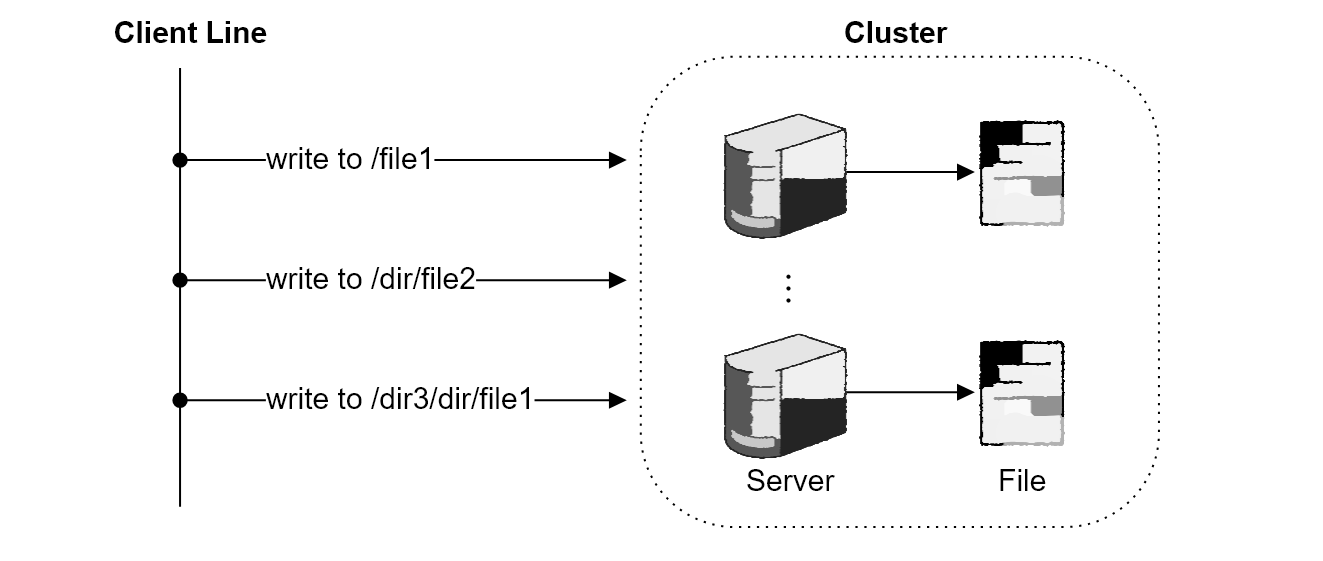
\includegraphics[width=\textwidth]{Sections/gfs/gfs.png}
  \caption{A high-level sketch of the Google File System (GFS) architecture.}
  \label{fig:gfs-architecture}

\end{figure}

\vspace{1em}
\noindent
\textbf{Note}: This is important as Google at the time was using cheap commodity hardware, which was prone to failure.

\newpage 

\noindent
The following details how files are stored in GFS:

\begin{Def}[File Chunking]

  Files in GFS are divided into \underline{fixed-size chunks} of 64MB.
  Each chunk is stored in a \textbf{chunk server}, identified by a unique 64 bit ID called a \textbf{chunk handle}.

  \underline{To ensure fault tolerance,} each chunk is \textbf{replicated} at least $N$ times across different chunk servers (Typically $N=3$).
\end{Def}

\begin{figure}[h]
  \centering
  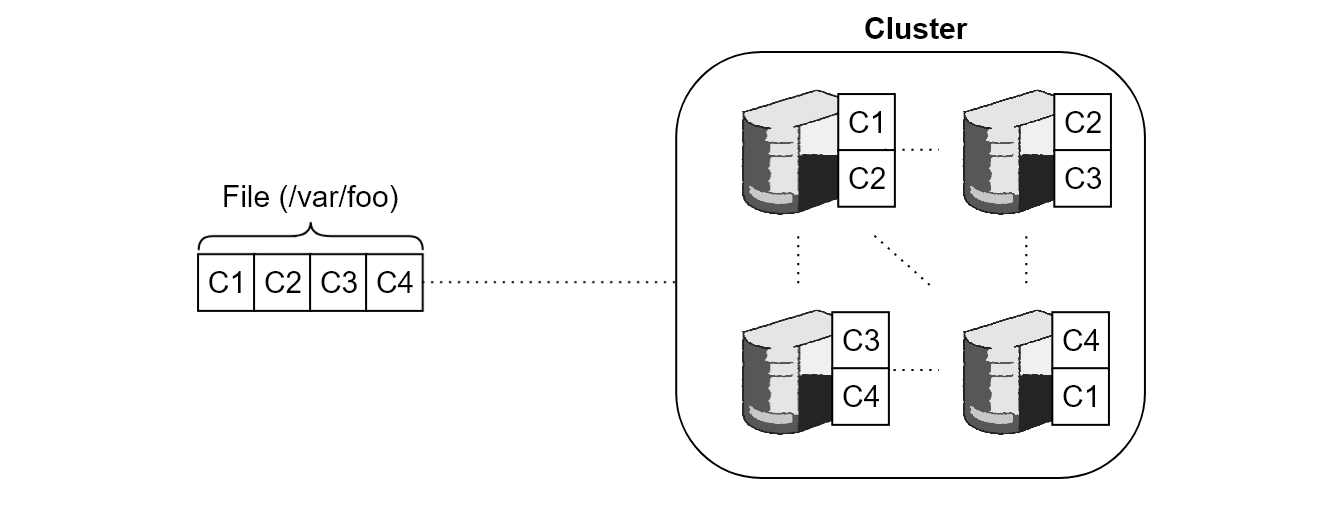
\includegraphics[width=\textwidth]{Sections/gfs/chunk.png}
  \caption{Simplified view of chunking in GFS, where a file is divided into 4 chunks (C1--C4), replicated twice across different servers.}
  \label{fig:gfs-chunking}
\end{figure}


\noindent
We decide to store metadata on a dedicated server to act as our coordinator.
\begin{Def}[Metadata Management]

  The GFS \textbf{master} serves \textbf{one cluster}, storing the following metadata in memory:
  \begin{itemize}
    \item \textbf{File \& Chunk Namespaces:} Hierarchical directory tree of files and the global chunk-ID namespace.
    \item \textbf{File$\to$Chunk Mapping:} For each file, the ordered list of chunk handles.
    \item \textbf{Chunk Replica Locations:} For each chunk handle, the set of chunkservers (IP:port) holding its replicas.
    \item \textbf{Access Control Information:} File permissions and ownership attributes.
  \end{itemize}
  
  \noindent
  In particular, mappings are persisted via an operation log. 
  Chunk locations are reconstructed by polling chunk servers at startup or when they join.
\end{Def}




\newpage

\noindent
Now to discuss how client's interact with the GFS system:
\begin{Def}[Client Interaction]

  \textbf{Clients} interact with GFS via a \underline{two-step process}:
  \begin{itemize}
    \item \textbf{Metadata Operations:} Clients query the master with the file name and chunk index, receiving the chunk handle and its replica locations.
    \item \textbf{Data Operations:} Clients then directly communicate with the chunk servers to read/write data.
  \end{itemize}
\end{Def}

\begin{figure}[h]
  \centering
  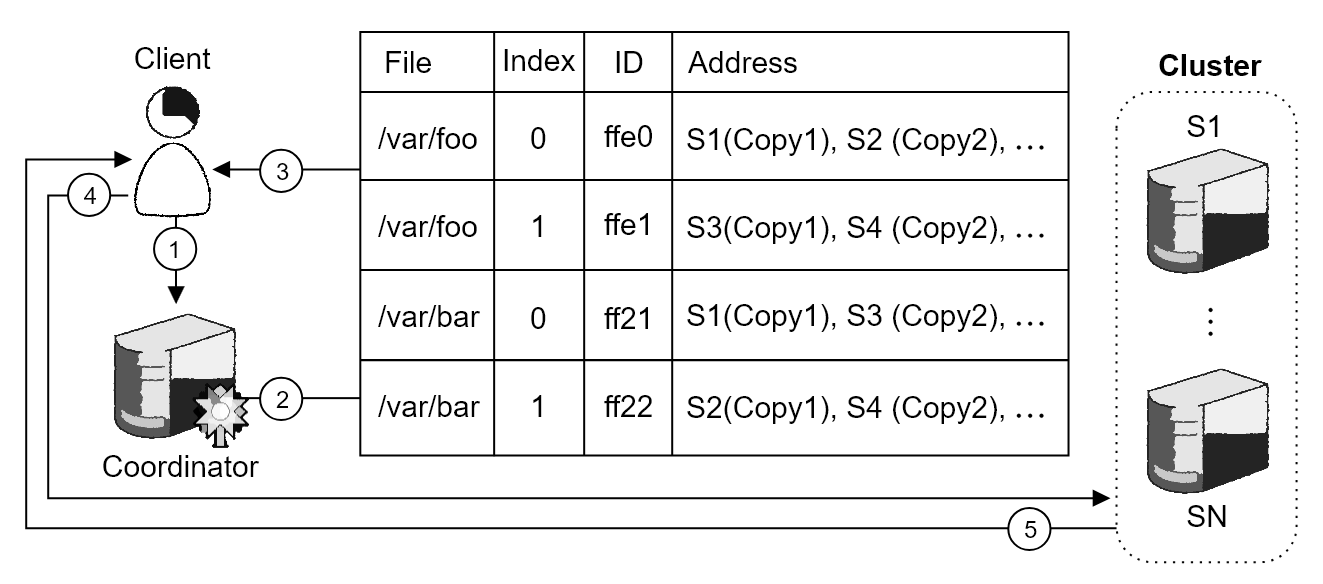
\includegraphics[width=\textwidth]{Sections/gfs/interaction.png}
  \caption{A Simplified view of client interaction with GFS. (1) Client sends a request to the master for metadata. (2) The master finds the chunk handle and its replica locations. 
  (3) The master returns the chunk handle and replica locations to the client. (4) The client sends a request to the chunk server for data. (5) The chunk server returns the data to the client.}
  \label{fig:gfs-client}
\end{figure}



    